% Created by tikzDevice version 0.12.3.1 on 2020-07-07 22:56:56
% !TEX encoding = UTF-8 Unicode
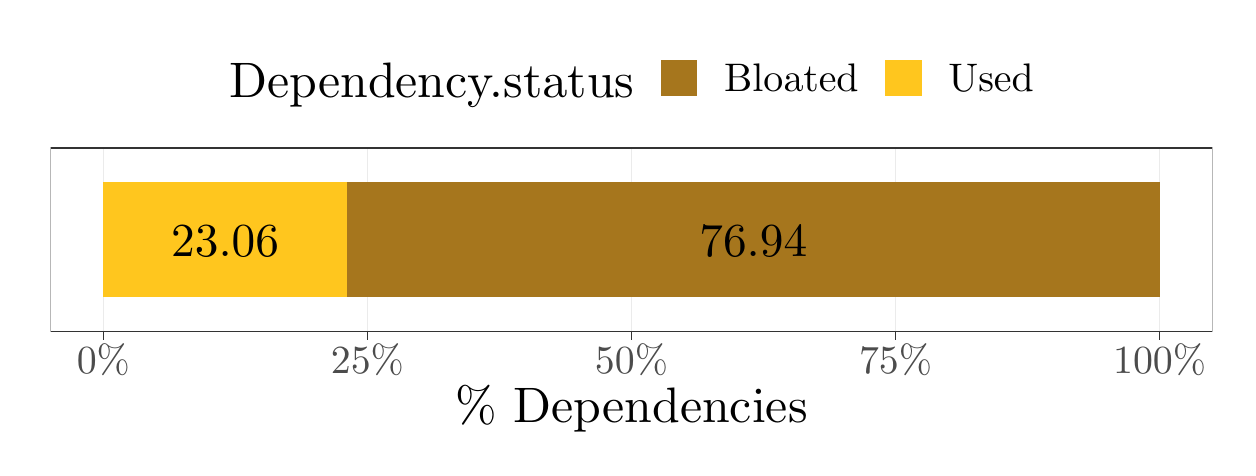
\begin{tikzpicture}[x=1pt,y=1pt]
\definecolor{fillColor}{RGB}{255,255,255}
\path[use as bounding box,fill=fillColor,fill opacity=0.00] (0,0) rectangle (433.62,151.77);
\begin{scope}
\path[clip] (  0.00,  0.00) rectangle (433.62,151.77);
\definecolor{drawColor}{RGB}{255,255,255}
\definecolor{fillColor}{RGB}{255,255,255}

\path[draw=drawColor,line width= 0.6pt,line join=round,line cap=round,fill=fillColor] (  0.00,  0.00) rectangle (433.62,151.77);
\end{scope}
\begin{scope}
\path[clip] (  8.25, 41.81) rectangle (428.12,108.37);
\definecolor{fillColor}{RGB}{255,255,255}

\path[fill=fillColor] (  8.25, 41.81) rectangle (428.12,108.37);
\definecolor{drawColor}{gray}{0.92}

\path[draw=drawColor,line width= 0.6pt,line join=round] ( 27.34, 41.81) --
	( 27.34,108.37);

\path[draw=drawColor,line width= 0.6pt,line join=round] (122.76, 41.81) --
	(122.76,108.37);

\path[draw=drawColor,line width= 0.6pt,line join=round] (218.18, 41.81) --
	(218.18,108.37);

\path[draw=drawColor,line width= 0.6pt,line join=round] (313.61, 41.81) --
	(313.61,108.37);

\path[draw=drawColor,line width= 0.6pt,line join=round] (409.03, 41.81) --
	(409.03,108.37);
\definecolor{fillColor}{RGB}{255,198,30}

\path[fill=fillColor] ( 27.34, 54.29) rectangle (115.36, 95.89);
\definecolor{fillColor}{RGB}{166,118,29}

\path[fill=fillColor] (115.36, 54.29) rectangle (409.04, 95.89);
\definecolor{drawColor}{RGB}{0,0,0}

\node[text=drawColor,anchor=base,inner sep=0pt, outer sep=0pt, scale=  1.71] at ( 71.35, 69.21) {23.06};

\node[text=drawColor,anchor=base,inner sep=0pt, outer sep=0pt, scale=  1.71] at (262.20, 69.21) {76.94};
\definecolor{drawColor}{gray}{0.20}

\path[draw=drawColor,line width= 0.6pt,line join=round,line cap=round] (  8.25, 41.81) rectangle (428.12,108.37);
\end{scope}
\begin{scope}
\path[clip] (  0.00,  0.00) rectangle (433.62,151.77);
\definecolor{drawColor}{gray}{0.20}

\path[draw=drawColor,line width= 0.6pt,line join=round] ( 27.34, 39.06) --
	( 27.34, 41.81);

\path[draw=drawColor,line width= 0.6pt,line join=round] (122.76, 39.06) --
	(122.76, 41.81);

\path[draw=drawColor,line width= 0.6pt,line join=round] (218.18, 39.06) --
	(218.18, 41.81);

\path[draw=drawColor,line width= 0.6pt,line join=round] (313.61, 39.06) --
	(313.61, 41.81);

\path[draw=drawColor,line width= 0.6pt,line join=round] (409.03, 39.06) --
	(409.03, 41.81);
\end{scope}
\begin{scope}
\path[clip] (  0.00,  0.00) rectangle (433.62,151.77);
\definecolor{drawColor}{gray}{0.30}

\node[text=drawColor,anchor=base,inner sep=0pt, outer sep=0pt, scale=  1.44] at ( 27.34, 26.95) {0\%};

\node[text=drawColor,anchor=base,inner sep=0pt, outer sep=0pt, scale=  1.44] at (122.76, 26.95) {25\%};

\node[text=drawColor,anchor=base,inner sep=0pt, outer sep=0pt, scale=  1.44] at (218.18, 26.95) {50\%};

\node[text=drawColor,anchor=base,inner sep=0pt, outer sep=0pt, scale=  1.44] at (313.61, 26.95) {75\%};

\node[text=drawColor,anchor=base,inner sep=0pt, outer sep=0pt, scale=  1.44] at (409.03, 26.95) {100\%};
\end{scope}
\begin{scope}
\path[clip] (  0.00,  0.00) rectangle (433.62,151.77);
\definecolor{drawColor}{RGB}{0,0,0}

\node[text=drawColor,anchor=base,inner sep=0pt, outer sep=0pt, scale=  1.80] at (218.18,  9.00) {\% Dependencies};
\end{scope}
\begin{scope}
\path[clip] (  0.00,  0.00) rectangle (433.62,151.77);
\definecolor{fillColor}{RGB}{255,255,255}

\path[fill=fillColor] ( 67.29,119.37) rectangle (369.08,146.27);
\end{scope}
\begin{scope}
\path[clip] (  0.00,  0.00) rectangle (433.62,151.77);
\definecolor{drawColor}{RGB}{0,0,0}

\node[text=drawColor,anchor=base west,inner sep=0pt, outer sep=0pt, scale=  1.80] at ( 72.79,126.62) {Dependency.status};
\end{scope}
\begin{scope}
\path[clip] (  0.00,  0.00) rectangle (433.62,151.77);
\definecolor{fillColor}{RGB}{255,255,255}

\path[fill=fillColor] (228.21,126.31) rectangle (242.66,140.77);
\end{scope}
\begin{scope}
\path[clip] (  0.00,  0.00) rectangle (433.62,151.77);
\definecolor{fillColor}{RGB}{166,118,29}

\path[fill=fillColor] (228.92,127.02) rectangle (241.95,140.06);
\end{scope}
\begin{scope}
\path[clip] (  0.00,  0.00) rectangle (433.62,151.77);
\definecolor{fillColor}{RGB}{255,255,255}

\path[fill=fillColor] (309.25,126.31) rectangle (323.70,140.77);
\end{scope}
\begin{scope}
\path[clip] (  0.00,  0.00) rectangle (433.62,151.77);
\definecolor{fillColor}{RGB}{255,198,30}

\path[fill=fillColor] (309.96,127.02) rectangle (322.99,140.06);
\end{scope}
\begin{scope}
\path[clip] (  0.00,  0.00) rectangle (433.62,151.77);
\definecolor{drawColor}{RGB}{0,0,0}

\node[text=drawColor,anchor=base west,inner sep=0pt, outer sep=0pt, scale=  1.44] at (251.66,128.58) {Bloated};
\end{scope}
\begin{scope}
\path[clip] (  0.00,  0.00) rectangle (433.62,151.77);
\definecolor{drawColor}{RGB}{0,0,0}

\node[text=drawColor,anchor=base west,inner sep=0pt, outer sep=0pt, scale=  1.44] at (332.70,128.58) {Used};
\end{scope}
\end{tikzpicture}
